\chapter{\ifenglish Introduction\else บทนำ\fi}

\section{\ifenglish Project rationale\else ที่มาของโครงงาน\fi}
จากปัญหาที่พบเจอในการจัดการร้านค้าที่มีลูกค้าจำนวนมากและต้องการจ่ายเงินกับพนักงานเพื่อทำการเช็คเอาต์ การรอคิวที่นาน และ การใช้พื้นที่ในการรอคิวอาจจะทำให้ลูกค้าไม่พึงพอใจได้
และการที่ไม่อยากให้ลูกค้าต้องมาต่อแถวที่ยาว วิธีการหนึ่งคือทำให้ลูกค้าสามารถจ่ายเงินของสินค้าด้วยตัวเองได้ ( self-service ) เป็นการที่ลูกค้าบริการตนเองโดยการหยิบสินค้าและจ่ายเงินให้ทางร้านค้าด้วยตัวเอง  เช่นผ่านทาง promptpay qr code
ซึ่งในร้านค้าที่ให้ลูกค้าบริการตัวเอง ก็จะมีปัญหาในการจัดการสินค้าในร้านค้า เนื่องจากในบางครั้งมีสินค้าที่หมด เนื่องจากไม่ทราบว่าขายสินค้าชิ้นใดไปแล้วเท่าไหร่ เพราะไม่มีการจัดการสินค้าที่ดี
โดยส่วนใหญ่ร้านค้าที่เป็น  self-service พนักงานจะต้องคอยนับจำนวนสินค้าที่เหลืออยู่ภายในร้านเพื่อทราบว่าขายอะไรไปแล้ว  หรือ รอให้สินค้าประเภทนั้นๆหมด แล้วจึงค่อยเติม stock ในทีเดียว

ผู้จัดทําจึงพัฒนาระบบ self-service CapSnap ลดปัญหาการรอคิวของลูกค้าโดยการให้ลูกค้าสามารถบริการตนเองได้  โดยใช้ Computational Intelligence ในการแยกแยะสินค้า ซึ่งทำให้ลูกค้าไม่ต้องเลือกเพื่อบันทึกในระบบว่าซื้อสินค้าชนิดใด  และ สามารถช่วยให้ร้านค้าสามารถจัดการสินค้าได้อย่างมีประสิทธิภาพจากการเก็บบันทึกจำนวนการขายของสิ้นค้าแต่ละชนิด และ เพิ่มประสิทธิภาพในการบริหารจัดการสินค้าในร้านค้า เพิ่มประสบการณ์ของลูกค้า และ ร้านค้าที่ต้องการเป้น self-service และ ลดการที่พนักงานต้องมาคอยจัดการนับสินค้าภายในร้าน



\section{\ifenglish Objectives\else วัตถุประสงค์ของโครงงาน\fi}
\begin{enumerate}
    \item เพื่อช่วยให้ลูกค้าสามารถบริการตนเองในร้านค้าได้ และให้ร้านค้าสามารถตรวจสอบสินค้าที่ขายได้
    \item เพื่อพัฒนาระบบ แยกแยะชนิดสินค้าโดยใช้ Computational Intelligence ได้
    \item เพื่อสร้างเว็บไซต์และแอปโทรศัพท์เพื่อให้ผู้ใช้งานสามารถใช้งานระบบได้
\end{enumerate}

\section{\ifenglish Project scope\else ขอบเขตของโครงงาน\fi}
ข้อมูลที่ใช้ในการ train ระบบ  Computational Intelligence  ในการแยกแยะชนิดสินค้า 
มาจาก ร้านค้าห้อง 422 ในภาคคณะวิศวกรรมศาสตร์ สาขา มหาวิทยาลัยเชียงใหม่ โดยมีสินค้าประมาณ 100 ชนิด
% \subsection{\ifenglish Hardware scope\else ขอบเขตด้านฮาร์ดแวร์\fi}

% \subsection{\ifenglish Software scope\else ขอบเขตด้านซอฟต์แวร์\fi}

\section{\ifenglish Expected outcomes\else ประโยชน์ที่ได้รับ\fi}
\begin{enumerate}
    \item แอปโทรศัพท์ที่ลูกค้าสามารถแยกแยะชนิดสินค้าเพื่อให้ลูกค้าสามารถจ่ายเงินให้กับสินค้านั้นๆได้ด้วยตัวเอง โดยไม่ต้องคอยเลือกชนิดของสินค้านั้นๆ
    \item เว็บไซต์ที่แสดงจำนวนการขายของสิ้นค้าแต่ละชนิดเพื่อให้ร้านค้าสามารถจัดการสินค้าได้
\end{enumerate}
\section{\ifenglish Technology and tools\else เทคโนโลยีและเครื่องมือที่ใช้\fi}
\begin{enumerate}
    \item Python + aiortc : สำหรับพัฒนาในส่วนของ Backend   , การรับข้อมูล streaming จาก Application   , การฝึกสอนโมเดล , และการ classify Product
    โดยไม่ต้องคอยเลือกชนิดของสินค้านั้นๆ

    \item Laravel (Web Application Framework) : สำหรับพัฒนา Frontend ในส่วนหน้าเว็บไซต์ของร้านค้า web dashboard
    \item Flutter + webrtc  (Mobile Application Framework) : สำหรับพัฒนา Frontend  ในส่วน Application ในโทรศัพท์ของลูกค้า และใช้ webrtc  การ streaming ภาพจาก camera  ไปยัง Backend
    \item MongoDB : สำหรับเก็บข้อมูลชนิดของสินค้าที่เอาไว้ใช้ฝึกสอนโมเดล , ใช้ในการแสดงราคาบน Frontend  และเก็บจำนวนของสินค้าที่ขายไปแล้ว

\end{enumerate}
% \subsection{\ifenglish Hardware technology\else เทคโนโลยีด้านฮาร์ดแวร์\fi}

% \subsection{\ifenglish Software technology\else เทคโนโลยีด้านซอฟต์แวร์\fi}

\section{\ifenglish Project plan\else แผนการดำเนินงาน\fi}
\begin{table}[h]
    % 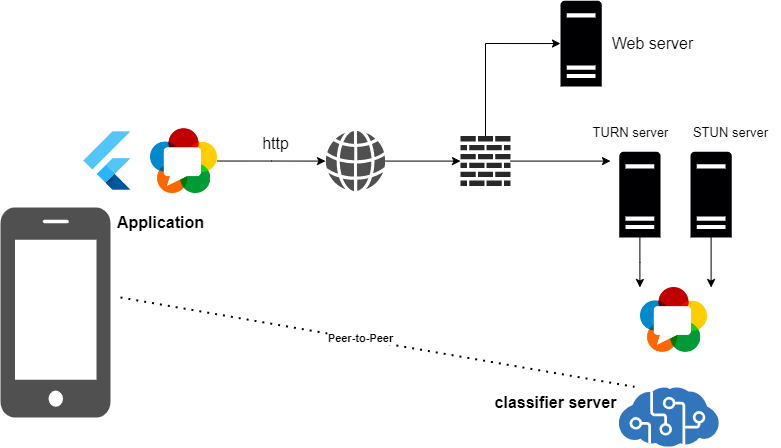
\includegraphics{pic/webrtc.png}
    \begin{plan}{1}{2023}{3}{2024}
        \planitem{1}{2023}{2}{2023}{Planning}
        \planitem{3}{2023}{3}{2023}{Document}
        \planitem{2}{2023}{3}{2023}{Back-end development}
        \planitem{5}{2023}{6}{2023}{App development}
        \planitem{11}{2023}{12}{2023}{Dashboard development}
        \planitem{1}{2024}{3}{2024}{Testing}
    \end{plan}
    
    \caption[Planning]{Planning}
    \label{table:Planning}
    \end{table}
 

\section{\ifenglish Roles and responsibilities\else บทบาทและความรับผิดชอบ\fi}
นายพงศกร รัตนพันธ์ รหัส 630610749 ทำในส่วนของ Backend การรับข้อมูล streaming จาก Application   , การฝึกสอนโมเดล , และการ classify Product  , เก็บข้อมูลรูปภาพของสินค้าและราคาลง MongoDB 

 และทำด้าน Application  ซึ่งใช้ webrtc  การ streaming ภาพจาก camera  ไปยัง Backend

นางสาวศุภริฎา  ศิลปสิทธิ์    รหัส  690610969 ทำในส่วนของ  Frontend ในส่วนหน้าเว็บไซต์ของร้านค้าที่แสดงข้อมูลจำนวนการขายสินค้าในแต่ละชนิดที่ขายไป web dashboard , เก็บข้อมูลรูปภาพของสินค้าและราคาลง MongoDB 
และ Frontend  ในส่วน Application ในโทรศัพท์ของลูกค้า 
\section{\ifenglish%
Impacts of this project on society, health, safety, legal, and cultural issues
\else%
ผลกระทบด้านสังคม สุขภาพ ความปลอดภัย กฎหมาย และวัฒนธรรม
\fi}

โครงการนี้ลดความซับซ้อนและเวลาที่ลูกค้าจะต้อง ไปรอต่อแถวเพื่อจ่ายเงินของสินค้า
รวมถึงทำให้พนักงานของร้านค้า ไม่ต้องคอยนับจำนวนสินค้าในร้านค้า  ในร้านค้าที่เป็นระบบ Self-Service  อีกทั้งยังเป็นอักทางเลือกหนึ่งในการที่ร้านค้าจะมาใช้ระบบ Self-Service ที่มีการจัดการที่ดี และ ส่งเสริมวัฒนธรรมในการบริการตนเองของลูกค้า
